%
% ─── CAPITULO 3: CONJUNTOS DE JULIA Y MANDELBROT ────────────────────────────────
%

Terminamos el capítulo \ref{chap:iteracion} fijándonos en la autosimilaridad de las imágenes que nos proporcionaba la aplicación del método de Newton en ciertas funciones complejas para deducir las cuencas de atracción de las distintas funciones. Pudimos comprobar que a pesar de ser imágenes que no son totalmente autosimilares, por lo que no son fractales en el sentido estricto, contienen fragmentos que sí lo son. Este mismo hecho se produce en los conjuntos de Julia y en el conjunto de Mandelbrot. Podemos observar este hecho en las imágenes \ref{fig:julia-intro}, que son nuestros primeros dos ejemplos de conjuntos de Julia.

\begin{figure}[ht]
    \centering
    \begin{tabular}{cc}
      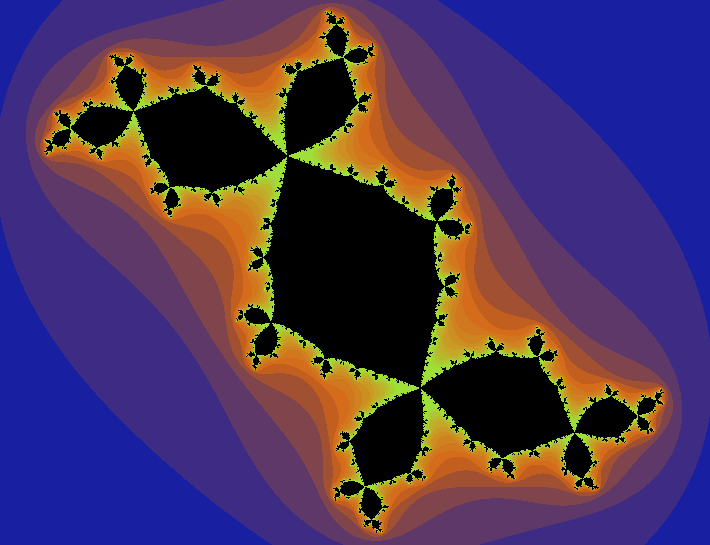
\includegraphics[scale=0.28]{./img/C3/julia-intro-2.png} &   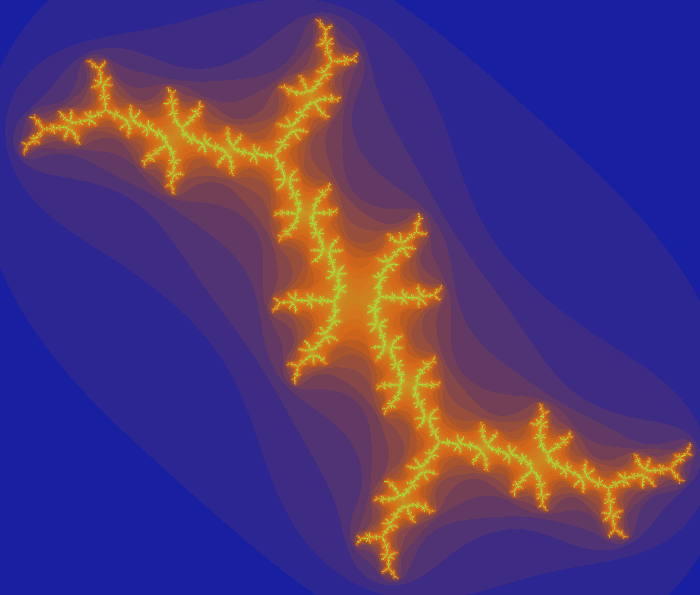
\includegraphics[scale=0.255]{./img/C3/julia-intro-1.png} \\
    (a) Conjunto de Julia conexo & (b) Conjunto de Julia no conexo  \\[6pt]
    \end{tabular}
    \caption{Primeras imágenes de conjuntos de Julia}
    \label{fig:julia-intro}
\end{figure}

Una notable diferencia entre las imágenes \ref{fig:julia-intro} se encuentra en que mientras en la imagen (a) se puede percibir cierta conexión en el conjunto, esta desaparece en el caso de la imagen (b). Precisamente en esa distinción reside la génesis del conocido \textit{conjunto de Mandelbrot}, que podemos también ver por primera vez, junto con algunas de sus autosimilaridades, en las imágenes \ref{fig:mandelbrot-intro}.

\begin{figure}[ht]
  \centering
  \begin{tabular}{cc}
    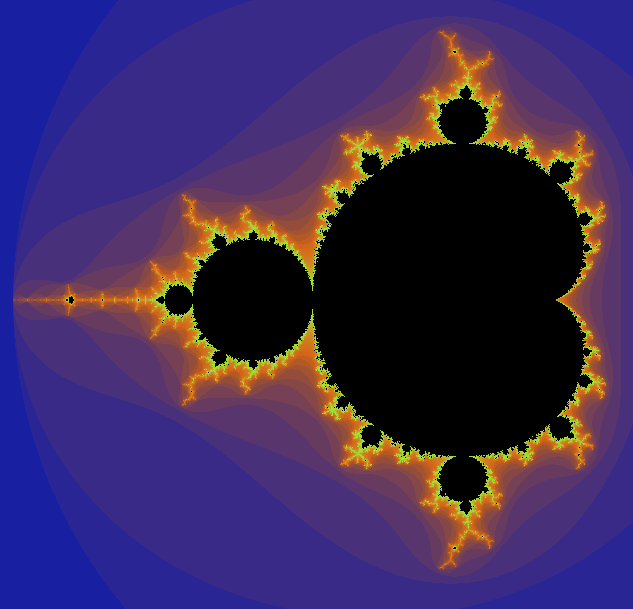
\includegraphics[scale=0.28]{./img/C3/mandelbrot-intro.png} &   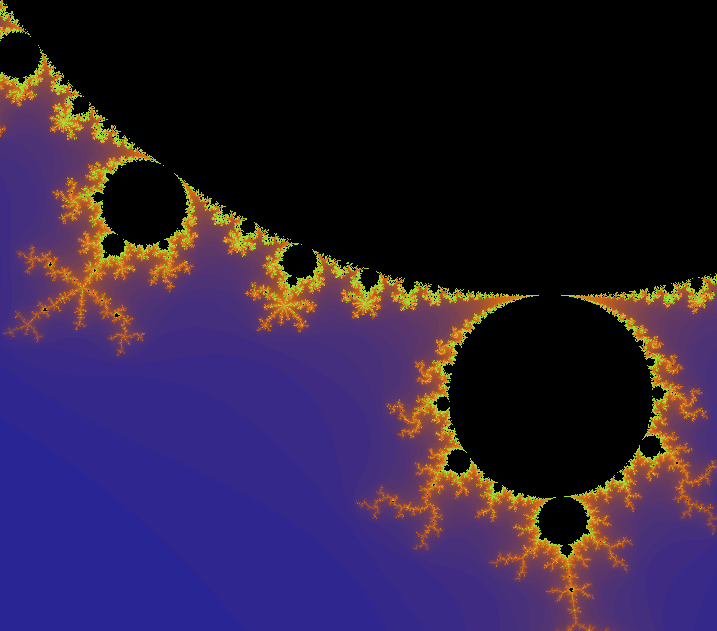
\includegraphics[scale=0.255]{./img/C3/detalle-Mandelbrot.png} \\
  (a) Conjunto completo & (b) Detalle ampliado  \\[6pt]
  \end{tabular}
    \caption{Primeras imágenes del conjunto de Mandelbrot}
    \label{fig:mandelbrot-intro}
\end{figure}

En este capítulo aprenderemos qué elementos componen estos conjuntos, y cómo llegar a visualizar estas imágenes tan llamativas.

\section{Iteración convergente y no convergente}

Recordamos que en el capítulo \ref{chap:iteracion}, a partir de una función analítica $f:\C\longrightarrow\C$, se le aplicaba una transformación $N_f(z)$ de forma que en muchos casos la iteración de dicha función era convergente independientemente del término $z_0\in\C$ inicial. Sin embargo recordemos que la iteración de una función cualquiera $f$ no siempre es convergente, como pudimos comprobar en el ejemplo situado al comienzo de la sección \ref{subsection:convergencia-punto-fijo}, en el que recordamos que las iteradas de la función $f(z)=z^2$ divergen siempre que $|z_0|>1$, convergen a $0$ si $|z_0|<1$ y quedan encerradas en $S^1$ en caso de que $|z_0|=1$. Otro posible comportamiento es el cíclico, como el que tienen las iteradas de la función $g(z)=z\cdot i$ en $z_0=1$, que si nos fijamos, son $O_g(1)=\{1,i,-1,-i,1,\dots\}$. 

Un último caso de posible comportamiento de una órbita son las órbitas caóticas, en las cuales no se percibe ningún patrón y además es muy sensible a las condiciones iniciales, fijémonos en lo que ocurre en el caso de la función $h(z)=z^2-1.9$ si miramos sus órbitas en $z_0=0,0.1$:

\begin{mmaCell}{Code}
  h[z_] := z^2 - 1.9;
  NestList[h, 0.1, 20]
  NestList[h, 0.0, 20]
\end{mmaCell}
\begin{mmaCell}{Output}
  \{0.1, -1.89, 1.6721, 0.895918, -1.09733, -0.695866,  \
  -1.41577, 0.104404, -1.8891, 1.6687, 0.884552, -1.11757, \
  -0.651043, -1.47614, 0.279, -1.82216, 1.42026, 0.117148, \
  -1.88628, 1.65804, 0.849092\}
\end{mmaCell}
\begin{mmaCell}{Output}
  \{0., -1.9, 1.71, 1.0241, -0.851219, -1.17543, -0.518374, \
  -1.63129, 0.761102, -1.32072, -0.155688, -1.87576, 1.61848, \
  0.719477, -1.38235, 0.0109007, -1.89988, 1.70955, 1.02256, \
  -0.854379, -1.17004\}
  \end{mmaCell}

No se observa ningún patrón de convergencia y además, a pesar de ser semillas muy cercanas, las órbitas son muy diferentes.

La dicotomía existente entre qué $z_0$ iniciales hacen que las iteradas de una función coverja, o no, restringida a cierta familia de funciones, es la que define a los distintos conjuntos de Julia. Presentamos por tanto, para cada $c\in\C$, la familia de funciones
\begin{equation}
  P_c(z) = z^2 +c \ \ \forall z\in\C.
\end{equation}

Nuestro objetivo es entonces clasificar para qué $z_0\in\C$, las iteradas $\{P_c^n(z_0)\}$ convergen, divergen, ciclan, o tienen posiblemente un comportamiento caótico.

\section{Conjuntos de Julia}
\label{section:Julia}

Sin dejar de tener en cuenta la familia de funciones $\{P_c(z)\}_{c\in\C}$ introducimos la siguiente definición.

\begin{definicion}
  Dado un número complejo $c\in\C$ fijo consideramos $P_c(z)=z^2+c$. Entonces:
  \begin{itemize}
    \item Se denomina \textbf{conjunto de puntos de escape}, y denotamos como $\mathsf{E}_c$, al conjunto de puntos cuyas iteradas divergen, es decir:
    $$
    \mathsf{E}_c = \{z_0\in\C: \{|P_c^n(z_0)|\}\rightarrow \infty \}
    $$
    \item  Se denomina \textbf{conjunto de puntos prisioneros}, y denotamos como $\mathsf{P}_c$ al conjunto de puntos cuyas iteradas no divergen, por lo que es el complemento de $\mathsf{E}_c$.
  \end{itemize}
\end{definicion}

A partir de estas dos definiciones, que insisten en clasificar exhaustivamente los puntos del plano complejo entre de escape o prisioneros según su órbita, podemos introducir la definición que esperábamos.

\begin{definicion}[Conjunto de Julia]
Dado un número $c\in\C$, se define su \textbf{conjunto de Julia}, y se denota como $\mathcal{J}_c$, a la frontera de $\mathsf{E}_c$. Se denomina \textbf{conjunto de Fatou} al complemento del conjunto de Julia.
\end{definicion}

Es precisamente en los complejos que pertenecen al conjunto de Julia donde las iteradas tienen un comportamiento caótico.

\begin{ejemplo}
  En el caso $c=0$, es decir, $P_0(z)=z^2$, sabemos ya que $\mathcal{J}_c=S^1$, pues precisamente es $S^1$ la frontera entre los puntos cuyas iteradas divergen o convergen a $0$.
\end{ejemplo}

\begin{observacion}
  Fijémonos por tanto que hay tantos conjuntos de Julia como números complejos, al poder asociar a cada número complejo un conjunto de puntos prisioneros, de escape, y por tanto un conjunto de Julia.
\end{observacion}

\subsection{Representación gráfica de los conjuntos de Julia}
\label{subsection:representacion-julia}

Tenemos entonces una definición de los conjuntos de Julia, pero aparentemente está muy alejada de las imágenes \ref{fig:julia-intro} que presentamos en la introducción. La forma de llegar a ellas es similar a la que utilizamos para graficar las imágenes que emplean la velocidad de convergencia en el capítulo \ref{chap:iteracion}. Sin embargo, y al contrario que al utilizar el método de Newton, ahora no tenemos ningún tipo de convergencia asegurada, por lo que el método de aplicar iteradas hasta encontrar un patrón no es el más correcto. Debemos por tanto encontrar una manera eficiente de clasificar cada punto del plano como prisionero o de escape. 

Para ello podemos fijarnos en que la operación de elevar $z_n$ al cuadrado prima sobre la de sumar una constante $c$ siempre que el módulo $|z_n|$ sea `suficientemente grande'. Procedemos entonces a enunciar el siguiente resultado:

\begin{teorema}
\label{th:escape}
  Dado un $c\in\C$, consideramos la función $P_c(z)=z^2+c$. Si un número $z_0\in\C$ verifica que $|z_0|>\max\{|c|,2\}$, entonces $z_0$ es un punto de escape. Al número $e_c=\max\{|c|,2\}$ se le denomina \textit{número de escape}.
\end{teorema}
\begin{proof}
  Supongamos que $|z_0|>e_c=\max\{|c|,2\}$, por tanto necesariamente debe existir un número $\varepsilon>0$ tal que $|z_0| = 2 + \varepsilon$. Aplicamos entonces la cadena de desigualdades siguiente:
  \begin{eqnarray*}
    |P_c(z_0)| = |z_0^2 + c| & \geq & |z_0^2| - |c|\text{  (propiedades del módulo)} \\
    & = & |z_0|^2 - |c| \\
    & \geq & |z_0|^2 - |z_0|\text{  (porque } |z_0|>|c| \text{)} \\
    & = & (|z_0|-1)|z_0| \\
    & = & (1 + \varepsilon)|z_0|.
  \end{eqnarray*}

  Por tanto tenemos que $|P_c(z_0)|\geq(1 + \varepsilon)|z_0|$, por lo que en cada iteración el módulo aumenta al menos $1+\varepsilon$ unidades, que es mayor que uno, es decir, $|P_c^k(z_0)|\geq(1+\varepsilon)^k|z_0|$, por lo que la sucesión diverge y $z_0$ es un punto de escape. 
\end{proof}

Podemos aplicar este teorema para programar un algoritmo que grafique conjuntos de Julia. Para ello, fijamos un número $M\in\N$ que será el máximo de iteraciones que se aplicarán en cada punto antes de decidir si el punto es prisionero o de escape. Si pasadas esas $M$ iteraciones el módulo de $z_0$ no ha alcanzado el número de escape $e_c$ entonces consideramos que $z_0$ es un punto prisionero. En caso contrario, en el momento que se alcance el número de escape cesarán las iteraciones y se etiquetará el punto como prisionero. El valor de $M$ puede ser alto si queremos aumentar la precisión a cambio de mayor tiempo de cómputo, y viceversa. Es posible que algunos de los puntos sean de escape pero alcancen $e_c$ después de las $M$ iteraciones, pero tomando un valor suficientemente alto el resultado es prácticamente el mismo.

Para graficar un conjunto de Julia podemos asignar un color fijo a los puntos prisioneros y a los puntos de escape asignarle otro en función de las iteraciones necesarias antes de alcanzar el número de escape. El psudocódigo del algoritmo descrito para graficar conjuntos de Julia sería el que podemos ver en el algoritmo \ref{alg:Julia}.

\begin{algorithm}[H]
  \caption{Conjuntos de Julia} \label{alg:Julia}
  \begin{algorithmic}
  \State Para cada $z_0\in\C$:
  \State $i\gets 0$
  \State $p\gets z_0$
  \While{$i < M$} 
    \State $p \gets P_c(p)$
    \If{$|p| > e_c=\max\{|c|,2\}$}
      \State break;
    \EndIf
    \State $i++$
  \EndWhile
  \If{$i=M$}
    \State $z_0$ es un punto prisionero
    \State \textbf{return} color de puntos prisioneros
  \Else
    \State $z_0$ es un punto de escape
    \State \textbf{return} color($i$)
  \EndIf
  \end{algorithmic}
\end{algorithm}

Por ejemplo, si queremos representar en \textit{Mathematica} el conjunto de la figura \ref{fig:julia-intro} (a), que era $\mathcal{J}_{-0.12+0.75i}$ utilizaríamos el siguiente código:

\begin{mmaCell}{Code}
  M = 50;
  Julia[z_, c_] := Length[FixedPointList[#^2 + c &, z, M, 
    SameTest -> (Abs[#] > Max[2.0, Abs[c]] &)]];
    
  DensityPlot[
    Julia[x + I y, -0.12 + 0.75 I], {x, -1.5, 1.5}, 
    {y, -1.25, 1.25}, PlotPoints->200, AspectRatio->Automatic, 
    ColorFunction -> (If[# >= 1, RGBColor[0, 0, 0], Hue[#]] &) ]
\end{mmaCell}

Fijémonos en que hemos utilizado el argumento \verb|SameTest| para especificar cuando dejar de iterar, especificando que se haga cuando se alcance $e_c$. Hemos utilizado también $M=50$ como máximo número de iteraciones. Podemos variar el segundo argumento de la llamada a la función \verb|Julia|, el rango de valores, el argumento \verb|PlotPoints| o el número máximo de iteraciones $M$ para graficar distintos conjuntos y detalles de los mismos. Algunos ejemplos de resultados de estos códigos se encuentran en la imagen \ref{fig:julia-explicados}.

\begin{figure}[ht]
  \centering
  \begin{tabular}{cc}
    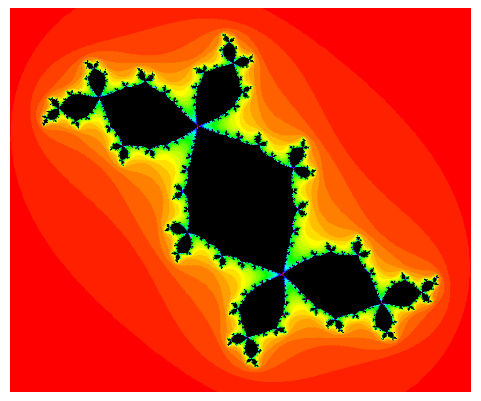
\includegraphics[scale=0.5]{./img/C3/julia-explicado-1.png} &   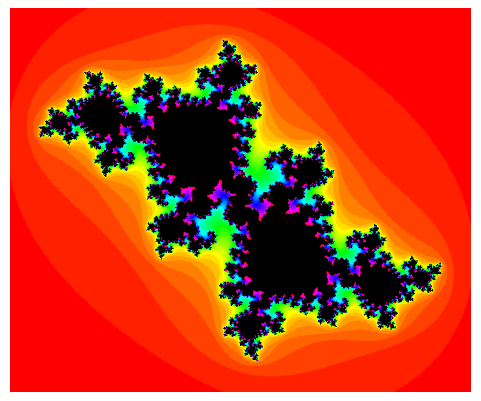
\includegraphics[scale=0.5]{./img/C3/julia-explicado-2.png} \\
  (a) $J_{-0.12+0.75i}$ & (b) $J_{-0.23+0.65i}$  \\[6pt]
  \end{tabular}
  \caption{Conjuntos de Julia graficados con Mathematica}
  \label{fig:julia-explicados}
\end{figure}

Por sí solo, Mathematica incluye una función \verb|JuliaSetPlot[c]| que muestra una imagen del conjunto $\mathcal{J}_c$. Esta función permite modificar los mismos parámetros que el método que acabamos de programar por nuestra cuenta\footnote{Más información en la documentación oficial: \url{https://reference.wolfram.com/language/ref/JuliaSetPlot.html?q=JuliaSetPlot}}, véanse las imágenes \ref{fig:julia-set-plot}.

\begin{figure}[ht]
  \centering
  \begin{tabular}{cc}
    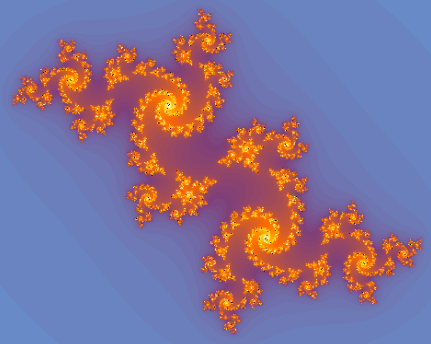
\includegraphics[scale=0.4]{./img/C3/juliaSetPlot-1.png} &   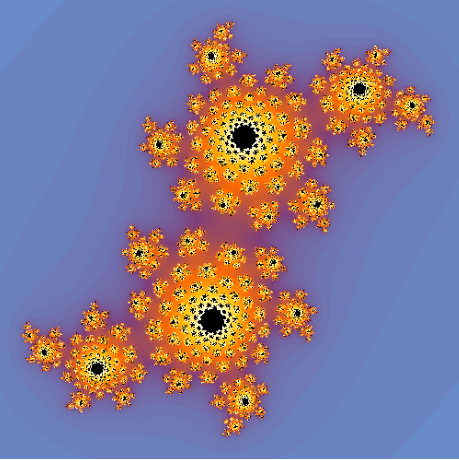
\includegraphics[scale=0.3]{./img/C3/juliaSetPlot-2.png} \\
  (a) $J_{-0.23+0.69i}$ & (b) $J_{0.16-0.59i}$  \\[6pt]
  \end{tabular}
  \caption{Resultados de la orden `JuliaSetPlot'}
  \label{fig:julia-set-plot}
\end{figure}

\section{Distinción entre conjuntos de Julia conexos y polvaredas}
\label{section:conexos-polvaredas}

Ya en la introducción de este capítulo y tras presentar las imágenes \ref{fig:julia-intro} prestamos atención a un detalle que, ahora que tenemos más ejemplos e imágenes de distintos conjuntos de Julia, se vuelve más evidente. Mientras algunos conjuntos de Julia se presentan conexos, como los de las imágenes \ref{fig:julia-explicados}, otros parecen no ser conexos y estar formados por trozos más pequeños, como los de las imágenes \ref{fig:julia-set-plot}. Cabe recordar que en realidad los conjuntos de Julia son la frontera entre los puntos que se representan en negro y los que se representan de colores.

Para saber qué conjuntos de Julia son conexos y cuales no \textit{Gaston Julia} y \textit{Pierre Fatou} demostraron en 1918 el siguiente teorema, cuya prueba se puede encontrar en \cite[Theorem 9.5]{John-Milnor}.

\begin{teorema}[Teorema de Fatou-Julia]
  \label{th:fatou-julia}
  Si $\mathsf{P}_c$ contiene todos los puntos críticos de $P_c(z)$, entonces $\mathcal{J}_c=\partial \mathsf{P}_c$ es conexo. Si al menos un punto crítico de $P_c(z)$ pertenece a $\mathsf{E}_c$, entonces $\mathcal{J}_c$ es isomorfo al conjunto de Cantor, es decir, tiene un conjunto no numerable de componentes conexas. 
\end{teorema}

En este último caso el conjunto de Julia se conoce como <<polvo de Fatou>>. En realidad el teorema en su versión original está enunciado para polinomios de grado mayor o igual que $2$, entendiendo las extensiones naturales del conjunto de puntos de escape y prisioneros. Si nos restringimos entonces a la familia $\{P_c(z)\}_{c\in\C}$, es muy sencillo caracterizar qué conjuntos de Julia son conexos y cuales son polvaredas.

\begin{corolario}
  \label{th:conexo-polvareda}
  Dado $c\in\C$, el conjunto de Julia $\mathcal{J}_c$ es conexo (resp. polvareda) si, y solo si, la sucesión de iteradas $\{P_c^n(0)\}$ no diverge (resp. diverge), es decir, si $0\in\mathsf{P}_c$ (resp. $0\in\mathsf{E}_c$).
\end{corolario}
\begin{proof}
  Es claro que $P'_c(z)=(z^2+c)'=2z$, por lo que los puntos críticos de $P_c(z)$ se alcanzan cuando $z=0$, por lo que aplicando el teorema \ref{th:fatou-julia} tenemos el resultado.
\end{proof}

Sobre la dicotomía entre qué conjuntos de Julia son conexos y cuales son polvareda surge el conocido \textbf{conjunto de Mandelbrot}, el cual adelantamos que está formado por los números complejos $c$ tales que su conjunto de Julia $\mathcal{J}_c$ es conexo. 

\section{El conjunto de Mandelbrot}
\label{section:Mandelbrot}

Como ya veníamos anunciando al final de la sección \ref{section:conexos-polvaredas}, el conjunto de Mandelbrot está formado por los $c\in\C$ tales que $\mathcal{J}_c$ es conexo. La idea inicial de \textit{Benoit Mandelbrot} para graficar el conjunto que denotaremos a partir de ahora como $\mathcal{M}$ fue pintar de negro los puntos del plano cuyo conjunto de Julia fuese conexo y de blanco el resto. De entrada parece una tarea titánica graficar, para cada punto del plano (aunque realmente sería solo un subconjunto suficientemente representativo), su conjunto de Julia y decidir si éste es o no conexo, pues en algunos casos la decisión se torna muy complicada.

Afortunadamente, gracias al teorema \ref{th:fatou-julia} y al corolario \ref{th:conexo-polvareda} esta tarea se vuelve mucho más sencilla, tan solo habría que tomar las iteradas en el origen, es decir $\{P_c^n(0)\}=\{c, c^2+c, (c^2+c)^2+c, \dots\}$ y decidir si la sucesión diverge o no mediante algún método similar al utilizado para graficar conjuntos de Julia.

Por resumir, de momento sabemos que:
\begin{eqnarray*}
  \mathcal{M} & = & \{c\in\C : \mathcal{J}_c \text{ es conexo }\} \\
              & = & \{c\in\C : 0\in\mathsf{P}_c \} \\
              & = & \{c\in\C : \{P_c^n(0)\}\not\rightarrow\infty\}
\end{eqnarray*}

\subsection{Representación gráfica del conjunto de Mandelbrot}
\label{subsection:representacion-mandelbrot}

Buscamos ahora obtener alguna figura similar a la imagen \ref{fig:mandelbrot-intro} a partir del conocimiento que tenemos de $\mathcal M$. Como ya viene siendo costumbre, la idea es dividir el plano en una cantidad finita de píxeles, asignando a cada uno un número complejo $c$ y evaluar en cada uno si la órbita en $z=0$ converge o diverge. Para tomar esta decisión nos podemos apoyar en el teorema \ref{th:escape} para probar este resultado.

\begin{proposicion}
  \label{prop:mandelbrot-escape}
  Dado un número complejo $c\in\C$, si $|c|>2$ entonces la sucesión de iteradas $\{P_c^n(0)\}$ es divergente.
\end{proposicion}
\begin{proof}
  Consideramos la sucesión de iteradas $z_0 = 0, z_n=P_c^n(0)$. Partimos de que $|c|>2$, por lo que buscamos encontrar un $m\in\N$ tal que $|z_m|>e_c=\max\{|c|,2\}=|c|$.
  
  Tenemos que $z_1=P_c(0)=c$, pero $|z_1|=|c|\not>|c|$.
  
  Si iteramos una vez más, $z_2=P_c^2(0)=P_c(c)=c^2+c$. Ayudándonos de una propiedad del módulo tenemos que:
  \begin{eqnarray*}
    |c^2+c| & \geq & ||c^2|-|c|| \\
            & = & ||c|^2 -|c|| \\
            & = & |c|^2-|c| \text{ (Pues al ser } |c|>2, |c|^2>|c|) \\
            & = & (|c|-1)|c|.
  \end{eqnarray*}
  Y como $|c|>2\Leftrightarrow |c|-1>1$, concluimos que
  $$
  |z_2|=|c^2+c| > |c| = \max\{|c|,2\} = e_c.
  $$
  Por lo que aplicando el teorema \ref{th:escape}, la sucesión $\{z_n\}$ es divergente.
\end{proof}

Este resultado nos facilita mucho la elaboración de un algoritmo que grafique a $\mathcal{M}$, pues de entrada nos afirma que todo número complejo cuyo módulo sea superior a $2$ no pertenece a $\mathcal M$. O dicho de otra forma, 
$$
\mathcal{M}\subseteq \{c\in\C: |c|\leq 2\} = \bar D(0,2),
$$
donde $D(z,r)$ denota el disco abierto de centro $z$ y radio $r$ mientras que $\bar D(z,r)$ denota el cierre del disco abierto, es decir, el disco cerrado de centro $z$ y radio $r$.

Además, en el momento que una iterada se sitúe fuera de $\bar D(0,2)$, podemos asegurar que esa sucesión va a diverger, por lo que podemos dejar de iterar. Para concluir que la sucesión no diverge, al igual que para graficar conjuntos de Julia, fijamos un número máximo de iteraciones $M\in\N$, de forma que si al calcular la $M$-ésima iterada el módulo del elemento $P_c^{M}(0)$ no ha excedido a $2$, podemos considerar que el número $c$ pertenece a $\mathcal{M}$. En conclusión, el algoritmo consiste en, para cada píxel identificado con un punto del plano complejo $c\in\C$, calcular sus iteradas hasta un máximo de $M$ iteraciones, en caso de exceder en módulo a $2$ guardamos el mínimo valor $m\in\N$ tal que $|P_c^m(0)|>2$ y asignamos un color en función; en caso de no exceder a $2$ asignar un color fijo. Presentamos por tanto en el algoritmo \ref{alg:Mandelbrot} el procedimiento para graficar el conjunto de Mandelbrot. 

\begin{algorithm}[H]
  \caption{Conjunto de Mandelbrot} \label{alg:Mandelbrot}
  \begin{algorithmic}
  \State Para cada $c\in\C$:
  \State $i\gets 0$
  \State $p\gets c$
  \While{$i < M$} 
    \State $p \gets P_c(p)$
    \If{$|p| > 2$}
      \State break;
    \EndIf
    \State $i++$
  \EndWhile
  \If{$i=M$}
    \State $c\in\mathcal{M}$
    \State \textbf{return} color de puntos de $\mathcal{M}$
  \Else
    \State $c\not\in\mathcal{M}$
    \State \textbf{return} color($i$)
  \EndIf
  \end{algorithmic}
\end{algorithm}

El código en \textit{Mathematica} utilizado es por tanto el siguiente, muy similar al utilizado para graficar conjuntos de Julia:

\begin{mmaCell}{Code}
  M = 100; 
  Mandelbrot = Compile[{{c, _Complex}}, 
    Length[FixedPointList[#^2 + c &, 0, M, 
    SameTest -> (Abs[#] > 2.0 &)]]];

  DensityPlot[Mandelbrot[x + I y], {x, -2.1, .7}, {y, -1.2, 1.2}, 
    Mesh -> False, Frame -> False, PlotPoints -> 200, 
    AspectRatio -> Automatic, 
    ColorFunction -> (If[# >= 1, Hue[0, 0, 0], Hue[#]] &)]
\end{mmaCell}

Al igual que en el caso de los conjuntos de Julia, \textit{Mathematica} tiene una función preprogramada que grafica el conjunto de Mandelbrot, llamada \verb|MandelbrotSetPlot|, la cual admite varios argumentos opcionales, como la región a graficar, el máximo de iteraciones, resolución, etc.\footnote{Más información en la documentación oficial \url{https://reference.wolfram.com/language/ref/MandelbrotSetPlot.html}}. 

\begin{figure}[ht]
  \centering
  \begin{tabular}{cc}
    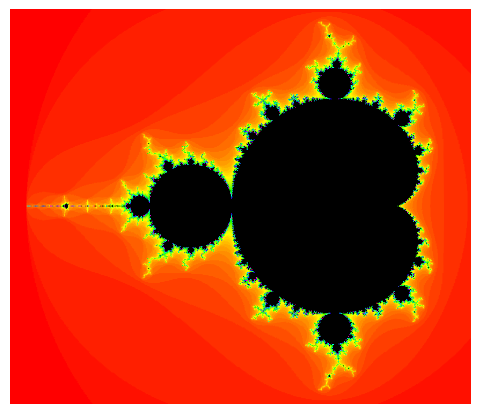
\includegraphics[scale=0.432]{./img/C3/Mandelbrot-Mathematica.png} &   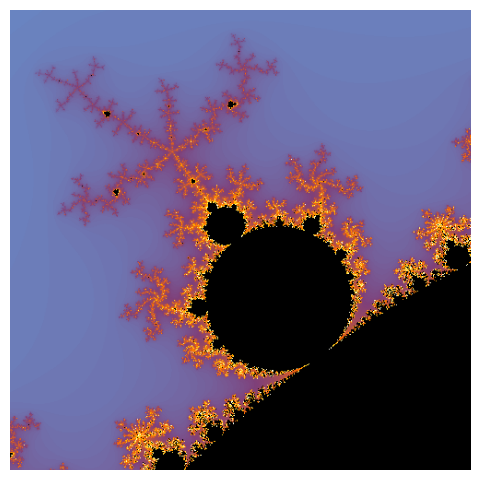
\includegraphics[scale=0.368]{./img/C3/MandelbrotSetPlot.png} \\
  (a) Salida del código \textit{Mathematica}  & (b) Salida de la orden `MandelbrotSetPlot' \\[6pt]
  \end{tabular}
  \caption{Representación de $\mathcal{M}$ y detalle en $[-0.65, -0.4]\times[0.47, 0.72]$}
  \label{fig:Mandelbrot-explicado}
\end{figure}

El conjunto de Mandelbrot es considerado por muchos como el objeto más complejo de la matemática. Además de la belleza que muestra por sí solo, los detalles de $\mathcal{M}$ esconden bonitas estructuras: bulbos, valles, antenas, copias reducidas del propio $\mathcal{M}$\dots

\section{Autosimilaridad de los conjuntos de Julia y Mandelbrot}
\label{section:autosimilaridad-julia-mandelbrot}

Ya en el comienzo de este capítulo mencionamos, y en las propias imágenes presentadas se puede comprobar, que los conjuntos de Julia y el conjunto de Mandelbrot no son objetos autosimilares, no al menos en el sentido de la definición \ref{def:autosimilaridad}. Sin embargo, sí contienen regiones y detalles que son autosimilares. En esta sección presentaremos algunas de las mismas.

\subsection{Autosimilaridad en conjuntos de Julia}

Recordemos el conjunto de Julia $\mathcal{J}_{-0.23+0.65}$, que podemos ver en la imagen \ref{fig:julia-explicados} (b). En las imágenes \ref{fig:detalles-julia} observamos distintos detalles, de forma que la primera es una ampliación de la original y las siguientes son cada una un `zoom' de la anterior.

Obsérvese cómo efectivamente las imágenes, salvo giro, son prácticamente iguales, pudiendo ver así una de las regiones autosimilares de $\mathcal{J}_{-0.23+0.65}$. En las imágenes \ref{fig:mas-detalles-julia} podemos ver algunas regiones ampliadas de ciertos conjuntos de Julia, pudiendo observar regiones autosimilares.

\newpage

\begin{figure}[ht]
  \begin{tabular}{ccc}
    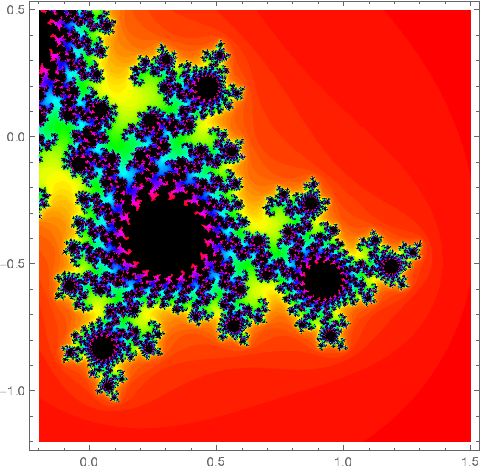
\includegraphics[scale=0.33]{./img/C3/julia-autosimilar-1.png} &   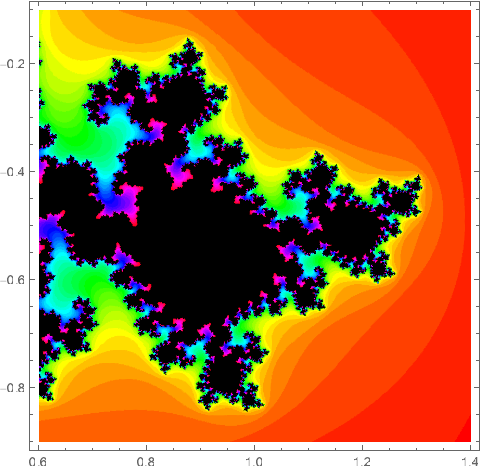
\includegraphics[scale=0.33]{./img/C3/julia-autosimilar-2.png} &   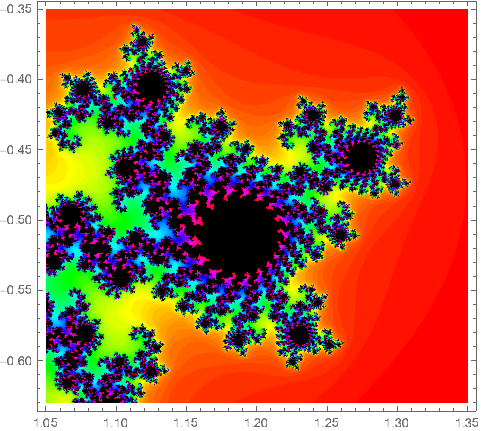
\includegraphics[scale=0.35]{./img/C3/julia-autosimilar-3.png} \\
  (a) $[-0.2,1.5]\times[-1.2,0.5]$ & (b) $[0.6,1.4]\times[-0.9,-0.1]$ & (c) $[1.05,1.35]\times[-0.65,-0.35]$ \\[6pt]
  \end{tabular}
  \caption{Diferentes regiones ampliadas de la figura \ref{fig:julia-explicados} (b)}
  \label{fig:detalles-julia}
\end{figure}

\begin{figure}[ht]
  \centering
  \begin{tabular}{cc}
    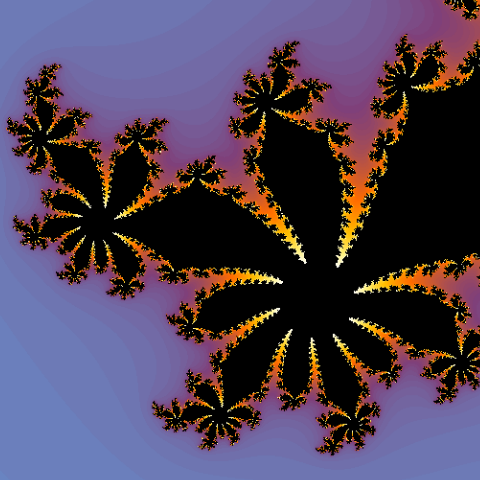
\includegraphics[scale=0.36]{./img/C3/julia-autosimilar-4.png} &   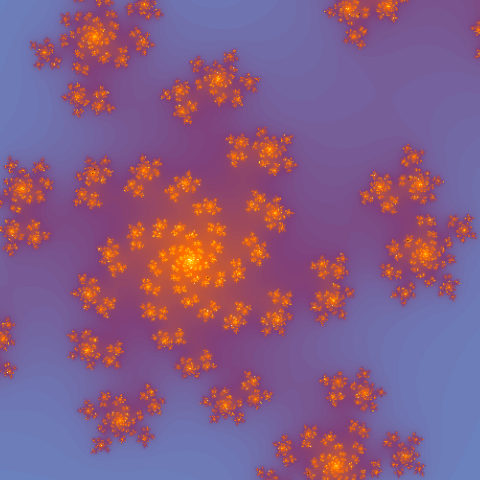
\includegraphics[scale=0.36]{./img/C3/julia-autosimilar-5.png} \\
  (a) $\mathcal{J}_{0.33-0.41 i}$ en $[-1,-0.3]\times[-1.1,-0.4]$ & (b) $\mathcal{J}_{0.48-0.13 i}$ en $[-0.6,-0.1]\times[0.25,0.75]$ \\[6pt]
  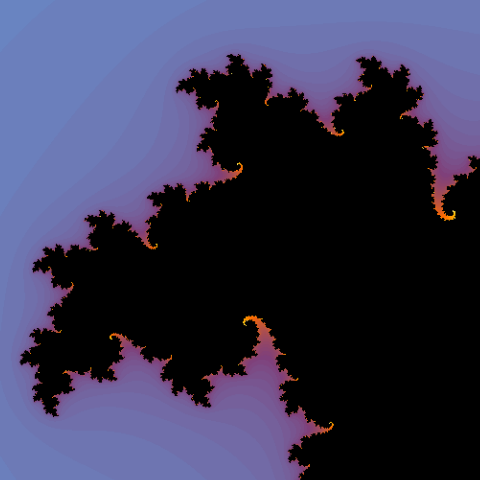
\includegraphics[scale=0.36]{./img/C3/julia-autosimilar-6.png} &   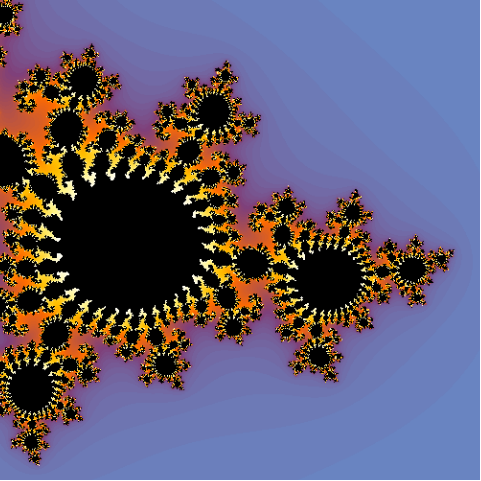
\includegraphics[scale=0.36]{./img/C3/julia-autosimilar-7.png} \\
  (c) $\mathcal{J}_{0.23+0.51i}$ en $[-1.1,-0.4]\times[0.4,1.1]$ & (d) $\mathcal{J}_{-0.52+0.51 i}$ en $[0,1.5]\times[-1,0.5]$ \\[6pt]
  \end{tabular}
  \caption{Detalles autosimilares de algunos conjuntos de Julia}
  \label{fig:mas-detalles-julia}
\end{figure}

\newpage

\subsection{Autosimilaridad en el conjunto de Mandelbrot}

El conjunto de Mandelbrot, el cual ya conocemos, está compuesto fundamentalmente de un cuerpo principal con forma de cardioide con gran cantidad de bulbos adosados al mismo (imagen \ref{fig:detalles-mandelbrot} (a), (b) y (d)), siendo cada uno de estos autosimilar y terminando en una antena que se bifurca (imagen \ref{fig:detalles-mandelbrot} (b) y (c)). Además, en el propio $\mathcal{M}$ hay minúsculas copias de sí mismo, en las cuales se vuelve a repetir su estructura (imagen \ref{fig:detalles-mandelbrot} (c)).

\begin{figure}[ht]
  \centering
  \begin{tabular}{cc}
    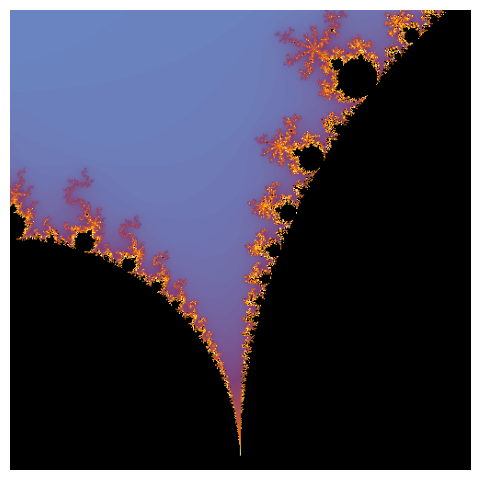
\includegraphics[scale=0.4]{./img/C3/mandelbrot-autosimilar-1.png} &   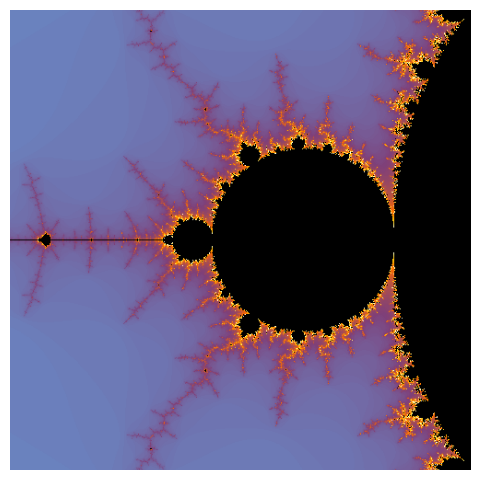
\includegraphics[scale=0.4]{./img/C3/mandelbrot-autosimilar-2.png} \\
  (a) $[-1,-0.5]\times[0,0.5]$ & (b) $[-1.5,-1.2]\times[-0.15,0.15]$ \\[6pt]
  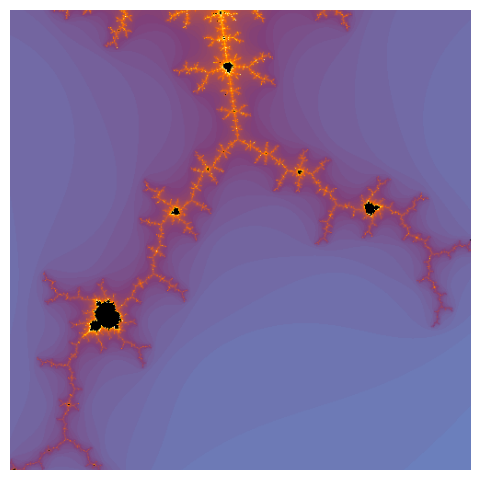
\includegraphics[scale=0.4]{./img/C3/mandelbrot-autosimilar-3.png} &   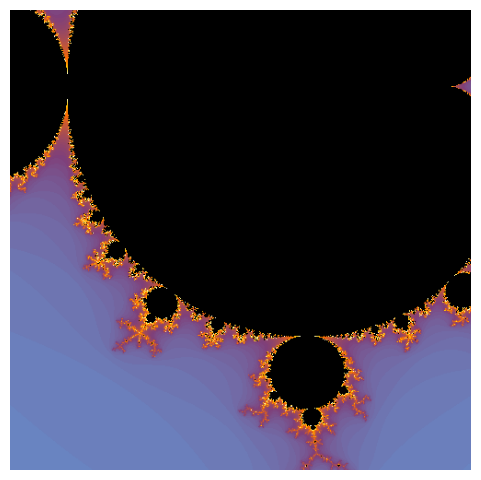
\includegraphics[scale=0.4]{./img/C3/mandelbrot-autosimilar-4.png} \\
  (c) $[-0.2,0]\times[-1.1,-0.9]$ & (d) $[-0.9,0.3]\times[-1,0.2]$ \\[6pt]
  \end{tabular}
  \caption{Detalles autosimilares de $\mathcal{M}$}
  \label{fig:detalles-mandelbrot}
\end{figure}

En la imagen \ref{fig:detalles-mandelbrot} (b) podemos ver una representación del que se conoce como `bulbo principal', pues es el más grande de todos los que están pegados al cuerpo principal. Podemos comprobar, observando los detalles que ofrecen las imágenes \ref{fig:detalles-bulbo}, que dicho bulbo muestra autosimilaridad.

\begin{figure}[ht]
  \centering
  \begin{tabular}{cc}
    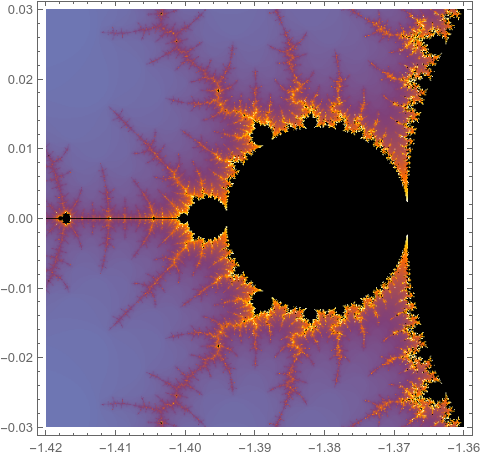
\includegraphics[scale=0.4]{./img/C3/mandelbrot-autosimilar-5.png} &   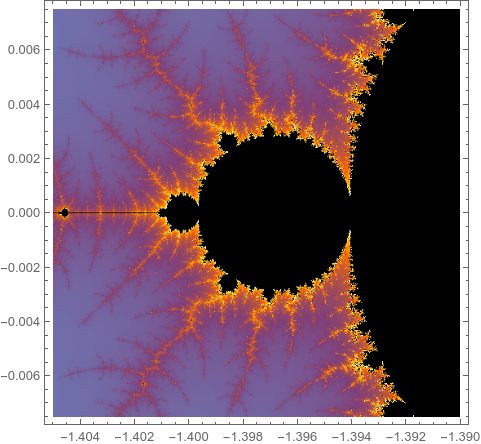
\includegraphics[scale=0.4]{./img/C3/mandelbrot-autosimilar-6.png} \\
  (a) $[-1.42,-1.36]\times[-0.03,0.03]$  & (b) $[-1.405,-1.39]\times[-0.0075,0.0075]$ \\[6pt]
  \end{tabular}
  \caption{Ampliaciones del bulbo principal de $\mathcal{M}$}
  \label{fig:detalles-bulbo}
\end{figure}

\section{Conjuntos de Julia y Mandelbrot generalizados}

Hasta el momento todo lo explicado y todas las imágenes obtenidas se han basado en la familia de funciones $\{P_c(z)\}_{c\in\C}=\{z^2+c\}_{c\in\C}$. Sin embargo, y como cabe esperar, la definición de los conjuntos de Julia como conjuntos frontera entre el conjunto de puntos prisioneros y de escape es completamente válido para las iteradas de cualquier función, o mejor dicho, para cualquier familia de funciones. En esta sección trataremos de extender los conocimientos obtenidos hasta ahora a otras funciones.

\subsection{Familia $\{z^m+c\}_{c\in\C}$}
\label{subsection:julia-mandelbrot-generalizados}

La extensión más natural y la que nos proporcionará resultados más llamativos consiste en cambiar el exponente de la función polinómica $P_c(z)$, a la cual ahora denotaremos como $P_{c,m}(z)=z^m+c$, con $m\geq 2$ natural para enfatizar el exponente. Es fácil comprobar que el teorema \ref{th:escape} es igual de válido con esta familia de funciones independientemente del exponente, por lo que el algoritmo sigue siendo el mismo, solo que en la función \verb|Julia| debemos cambiar el exponente. Además, la orden \verb|JuliaSetPlot| ya presentada en la sección \ref{subsection:representacion-julia} admite la posibilidad de indicarle una función arbitraria. Es esta la forma en la que hemos graficado las imágenes \ref{fig:julia-generalizados}.

\begin{figure}[ht]
  \centering
  \begin{tabular}{cc}
    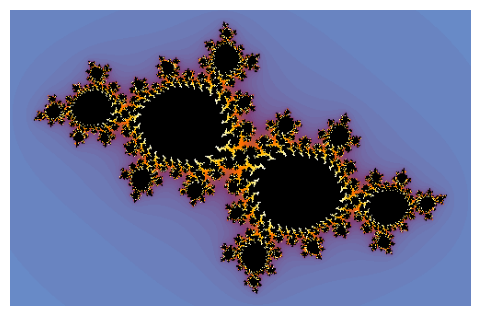
\includegraphics[scale=0.55]{./img/C3/julia-generalizado-2.png} &   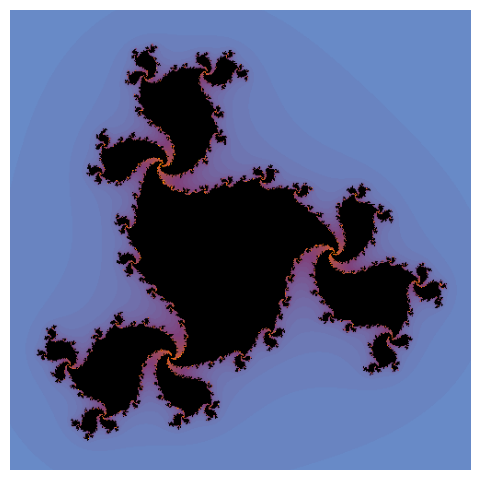
\includegraphics[scale=0.4]{./img/C3/julia-generalizado-3.png} \\
  (a) $z^2-0.55+0.48i$ & (b) $z^3-0.55+0.48i$ \\[6pt]
  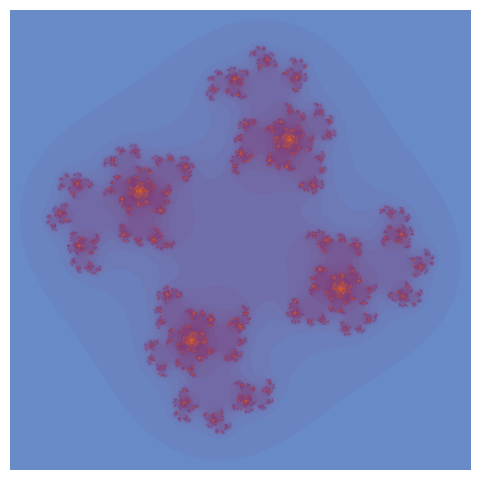
\includegraphics[scale=0.4]{./img/C3/julia-generalizado-4.png} &   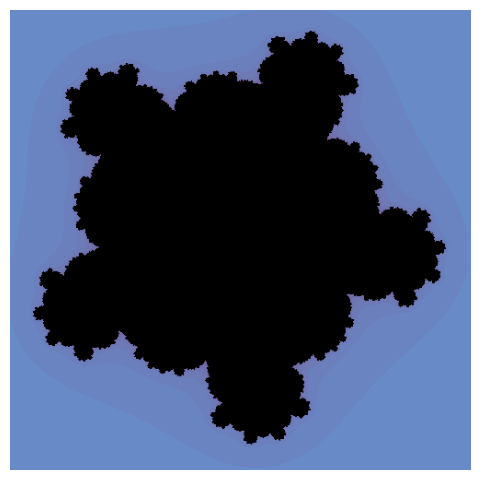
\includegraphics[scale=0.4]{./img/C3/julia-generalizado-5.png} \\
  (c) $z^4-0.55+0.48i$ & (d) $z^5-0.55+0.48i$ \\[6pt]
  \end{tabular}
  \caption{Conjuntos de Julia con $P_{-0.55+0.48i, m}$ para distintos valores de $m$.}
  \label{fig:julia-generalizados}
\end{figure}


Fijémonos en que hemos fijado $c=-0.55+0.48i$ y hemos variado el exponente de la función polinómica. Llama la atención lo distintos que son los conjuntos entre sí cuando realmente el $c$ fijado es el mismo en todos los casos. 

Como ya comentamos en la sección \ref{section:conexos-polvaredas}, el teorema \ref{th:fatou-julia} (teorema de la dicotomía de Fatou-Julia) es válido para cualquier polinomio de grado mayor o igual que 2, en particular es válido para la familia de funciones $\{P_{c,m}(z)\}_{c\in\C}$. Tenemos por tanto que de la misma forma es válido el corolario, por lo que la distinción entre conjuntos de Julia conexos y polvaredas se vuelve a basar en buscar la convergencia o divergencia de la sucesión $\{P_{c,m}^n(0)\}$.

De esta forma, podemos hablar por tanto de conjuntos de Mandelbrot generalizados como representación gráfica de qué puntos tienen un conjunto de Julia conexo o polvareda utilizando la función $P_{c,m}(z)$, el cual denotamos como $\mathcal{M}_m$. De la misma forma que el resultado \ref{th:escape} es válido en la generalización, la proposición \ref{prop:mandelbrot-escape} también lo es, por lo que podemos también reutilizar el código que empleamos para representar el conjunto de Mandelbrot con tan solo variar el exponente, ver imágenes \ref{fig:mandelbrot-generalizados}. Por su parte, la función de \textit{Mathematica} \verb|MandelbrotSetPlot| admite un argumento \verb|n| que representa el exponente de $P_{c,m}(z).$ a la hora de iterar.

\begin{figure}[ht]
  \centering
  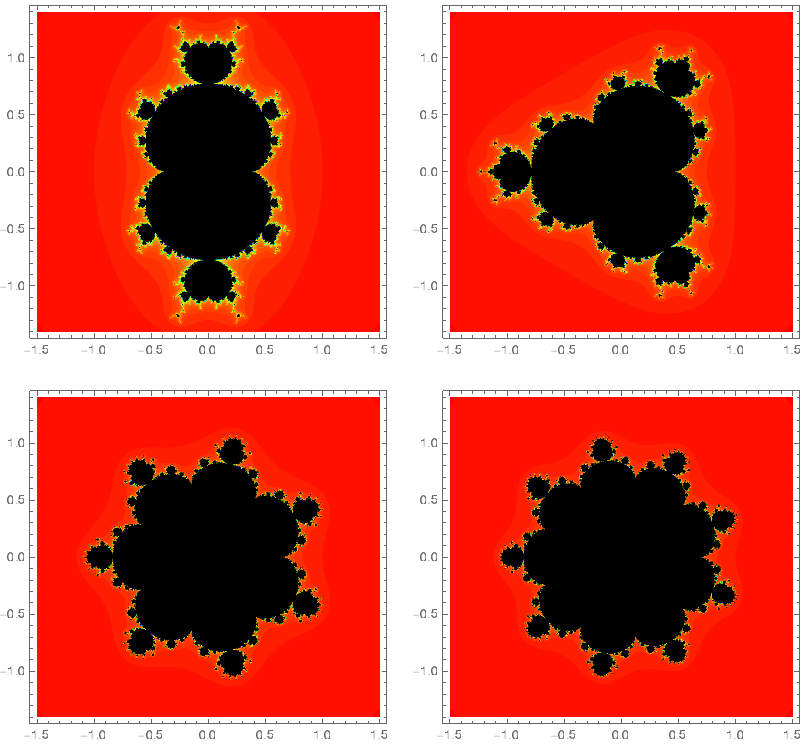
\includegraphics[scale=0.7]{./img/C3/mandelbrot-generalizado.png}
  \caption{Conjuntos de Mandelbrot $\mathcal{M}_m$ para $m=3,4,8,10$}
  \label{fig:mandelbrot-generalizados}
\end{figure}

Obsérvese que a pesar de encontrar cierta similaridad en la formas de los distintos conjuntos de Mandelbrot generalizados, podemos determinar puntos que para unos exponentes se encuentran dentro y en otros casos fuera de su respectivo $\mathcal{M}_m$. Este hecho explica lo ocurrido con $c=-0.55+0.48i$, que para ciertos exponentes el conjunto de Julia es conexo y para otros es polvareda.

Finalmente, invitamos al lector a visitar una web interactiva que hemos desarrollado como parte del TFG, la cual se describe minuciosamente su diseño e implementación a partir del capítulo \ref{chap:visualizacion}. En esta web es posible visualizar tantos conjuntos de Julia y Mandelbrot estándar y generalizados como desee, además de modificar dinámicamente parámetros como la constante $c$ de los conjuntos de Julia o hacer `zoom' a las distintas regiones para poder observar los detalles y entresijos que nos ofrecen los conjuntos de Julia y de Mandelbrot. Su url es \url{https://jantoniovr.github.io/Geometria-Fractal/}(WIP).%TODO Modificar si es necesario esta URL

\newpage
\subsection{Conjuntos de Julia con funciones no polinómicas}

Además de todos los conjuntos de Julia ya tratados y visualizados, utilizando otras funciones no polinómicas como pueden ser las trigonométricas y las exponenciales (complejas) también se pueden graficar algunos conjuntos con formas distintas a las ya vistas y con hermosas propiedades. A continuación mostraremos tan solo algunos ejemplos:
\newpage
\begin{itemize}
  \item Con la familia $f_c(z)=c\cdot \sin(z)$:
  
\begin{figure}[ht]
  \centering
  \begin{tabular}{cc}
    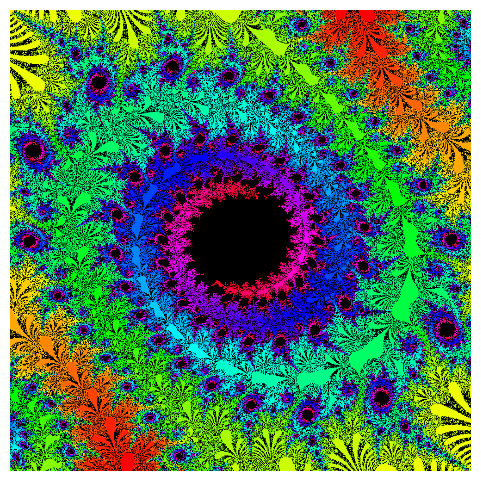
\includegraphics[scale=0.45]{./img/C3/juliaS-1.png} &   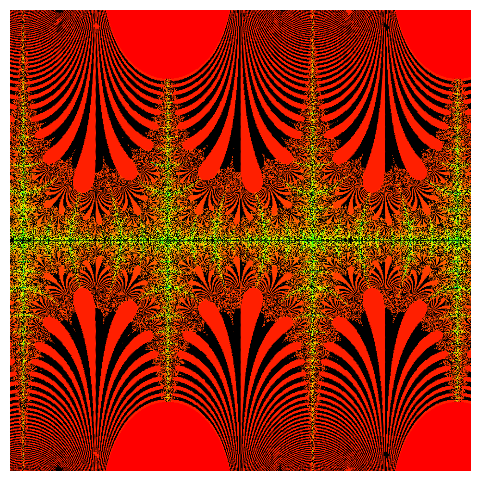
\includegraphics[scale=0.45]{./img/C3/juliaS-2.png}
  \end{tabular}
\end{figure}


\item Con la familia $f_c(z)=c\cdot \cos(z)$:
  
\begin{figure}[ht]
  \centering
  \begin{tabular}{cc}
    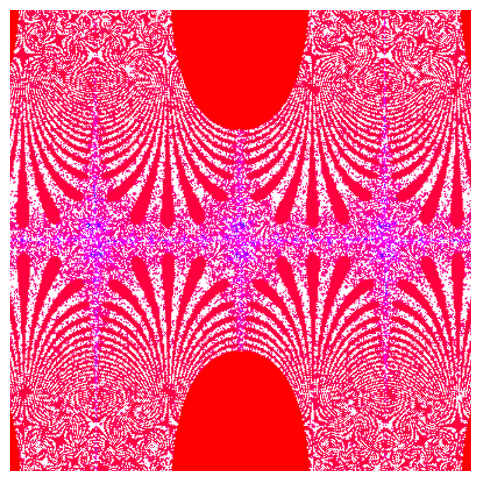
\includegraphics[scale=0.45]{./img/C3/juliaC-1.png} &   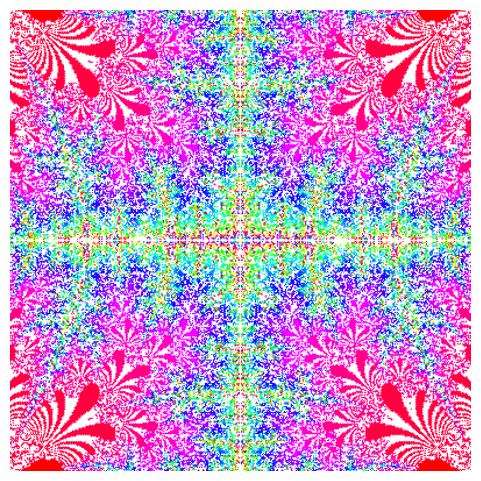
\includegraphics[scale=0.45]{./img/C3/juliaC-2.png}
  \end{tabular}
\end{figure}

\item Con la familia $f_c(z)=c\cdot e^z$:
  
\begin{figure}[ht]
  \centering
  \begin{tabular}{cc}
    
\includegraphics[scale=0.45]{./img/C3/juliaE-1.png} &   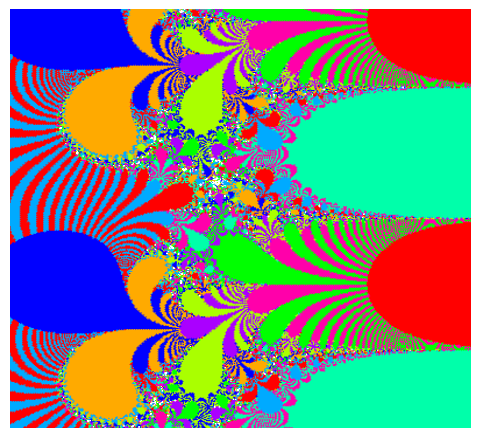
\includegraphics[scale=0.45]{./img/C3/juliaE-2.png}
  \end{tabular}
\end{figure}

\end{itemize}